\documentclass{article}


\usepackage{arxiv}

\usepackage[utf8]{inputenc} % allow utf-8 input
\usepackage[T1]{fontenc}    % use 8-bit T1 fonts
\usepackage{hyperref}       % hyperlinks
\usepackage{url}            % simple URL typesetting
\usepackage{booktabs}       % professional-quality tables
\usepackage{amsfonts}       % blackboard math symbols
\usepackage{nicefrac}       % compact symbols for 1/2, etc.
\usepackage{microtype}      % microtypography
\usepackage{lipsum}
\usepackage{graphicx}
\graphicspath{ {./figures/} }

\usepackage[backend=biber,
	style=numeric,
	bibencoding=utf8,
	natbib=true
	]{biblatex}
\addbibresource{references.bib} 


\title{3D U-Net for prostate MRI segmentation}


\author{
  Daniel Homola \\
  \texttt{dani.homola@gmail.com} \\
}

\begin{document}
\maketitle


\section{Introduction}
This mini project implements the fully convolutional 3D U-Net segmentation network \cite{_i_ek_2016} and traisn/evaluates it on the \href{https://goo.gl/fw8qku}{NCI-ISBI 2013 Challenge: Automated Segmentation of Prostate Structures} dataset, which consists of 80 patients' 3D MRI scans from their prostate region. The model was implemented using core TensorFlow (i.e. without Keras) and Python. The main focus of this work was establishing preliminary benchmark performance along with developing a package that enables us to quickly iterate and try various model architectures (through hyperparameter tuning) and evaluation methods. Therefore, the project, in its current form is not intended to be a rigorous and thorough evaluation of the algorithm and it is merely a platform for future work and experimentation.

\section{Data preparation}

The dataset's train and leadership samples were combined to form a training set of 70 samples. The number of scans, their dimensions and various other relevant sample metrics were explored using the \texttt{data\_exploration} jupyter notebook. Several of the MRI scans and their corresponding segmentation data were examined from different patients using tiled plots and animations. 

Finally, the scans were preprocessed using the following steps:

\begin{itemize}
	\item All MRI scans were rescaled to be between zero and one.
	\item Although the 3D U-Net is a fully convolutional network architecture (which is therefore dimension agnostic), the training scans were down-sampled to 128 x 128 size to reduce the required memory during training. The test dataset was saved in both original and resized sizes to ensure we measure test performance on the original resolution. 
	\item To form batches of the data at training time, the number of scans (i.e. the depth of input tensors) had to be unified across patients. Therefore, each patient's data was maximised to be no more than 32 scans. Then, at training time, patients with less scans are padded with zeros.
	\item An input size of [\texttt{batch}, 32, 128, 128, 1] was also desirable as the network has shortcut connections between the analysis and synthesis paths, which necessitate compatible tensor dimensions at equal depths of the architecture. Maximum depth of 32 was chosen, as the network's three dimensional max-pooling and up-convolutional operations both shrink and expand the data by a factor of 2 respectively. Therefore, an input tensor dimension that is the power of two guarantees error free batches without masking.
	\item Unfortunately, no time was left for incorporating data augmentation into the input pipeline which surely did hurt the performance of the trained models.
\end{itemize}


\section{Model architecture}

The original implementation was followed as closely as possible, including convolutional, max-pooling and transposed convolutional layer parameters. Batch normalisation \cite{ioffe2015batch} and softmax with weighted cross-entropy loss were also used as in the original paper. Due to the flexible parametrisation of experiments in this implementation, several crucial hyperparameters of the model architecture can be easily changed by changing a model's \texttt{params.json} file. These parameters include: depth of architecture, number of 3D convolutional filters to use in the first layer, and a flag for whether to use batch normalisation.

Furthermore, we can set the batch size, training steps, learning rate, class weights, train and test datasets to use as well from the model folder's parameter file.

Due to time constraints, only a few models were trained for this project (see below), and they were only trained for a short period of time (100 epochs). To see the full hyperparameter list of these referenced models, please check the \texttt{params.json} file in the project's \texttt{models}. 

\begin{itemize}
	\item \texttt{base\_model}: Mimics the original paper's architecture: \texttt{depth}=4, \texttt{n\_base\_filters}=32, \texttt{BN}=True.
	\item \texttt{base\_model\_no\_bn}: Same as above but without batch normalisation. 
	\item \texttt{deeper\_model}: \texttt{depth}=6, \texttt{n\_base\_filters}=8, \texttt{BN}=True.
\end{itemize}



\section{Model performance}

The performance of these models were assessed on the test dataset's 10 patients, using the mean Intersection of Union (IoU) across the three classes, defined as $\frac{TF}{TF + FP + FN}$, where TP: true positives, FP: false positives, FN: false negatives. Due to  time constraints, proper cross-validation was not carried out and the networks were only tested on this one test set. Similarly, (and unfortunately), the other interesting evaluation methods of the paper, such as artificially un-labelling some of the data and assessing model performance as a function of labelled slices, were also left out from this initial work. Some of these ideas would be relatively easy to incorporate given the current state of the project however.

Both the original test dataset (without resizing to 128x128) and the resized version were used for evaluation. With model \texttt{deeper}, the original 400x400 scans of the test dataset resulted in incompatible layer sizes, that could not been concatenated, hence the missing evaluation for this model-testset pair. As could be clearly seen from Table\ref{tab:table1}, there is quite a lot of room for improvement, compared to the authors' results. Nonetheless, and not surprisingly, the results demonstrate, that deeper architectures and batch normalisation get better results.

\begin{table}[!ht]

	\centering
	\begin{tabular}{lcc}
		\toprule
		{} & \multicolumn{2}{c}{\textbf{Mean IOU}}  \\
		\cmidrule(r){2-3}
		\textbf{Model}     & Original     & 128 x 128 \\
		\midrule
		Base with BN    & 0.3384  & 0.4731  \\
		Base w/o BN     & 0.3081  & 0.3284  \\
		Deeper with BN  & -  & 0.5223  \\
		\bottomrule
	\end{tabular}
	\vspace{3mm}
	\caption{Model performance on test dataset}
	\label{tab:table1}
\end{table}

Finally, Figure \ref{fig:fig1} and Figure \ref{fig:fig2} show segmented MRI images from the base model and deeper model respectively. Despite the poor overall performance, these images are actually quite encouraging and demonstrate that the models are heading/training in the right direction. We can generate tiled-plots like this (or even animations) for any of the patients from any of our models, see \texttt{model\_exploration} notebook. 

\section{Software engineering decision}

The project was built around the excellent high-level \texttt{tf.data} and \texttt{tf.estimator} APIs of TensorFlow.  The model itself was implemented using \texttt{tf.layers}. The best practices dictated by the general guides and tutorials of the official TensorFlow site were followed and respected wherever possible. Several TensorFlow anomalies/bugs (\href{https://github.com/tensorflow/tensorflow/issues/20379}{1}, \href{https://github.com/tensorflow/tensorflow/issues/21748}{2}, and others mentioned in the code) were encountered during development, but thanks to the strong community around TF most were fairly easy to resolve. 

Additionally, I took inspiration from the repo of \href{https://github.com/cs230-stanford/cs230-code-examples/tree/master/tensorflow/vision}{Stanford's CS230 class} and also used this \href{https://drivendata.github.io/cookiecutter-data-science/}{cookiecutter} template to start with. Unfortunately I did not have time left to write a few unit-tests for the data preprocessing and handling functionality. If I had had time for it, I would have chosen \texttt{pytest} for this.


\begin{figure}[t]
	\centering
	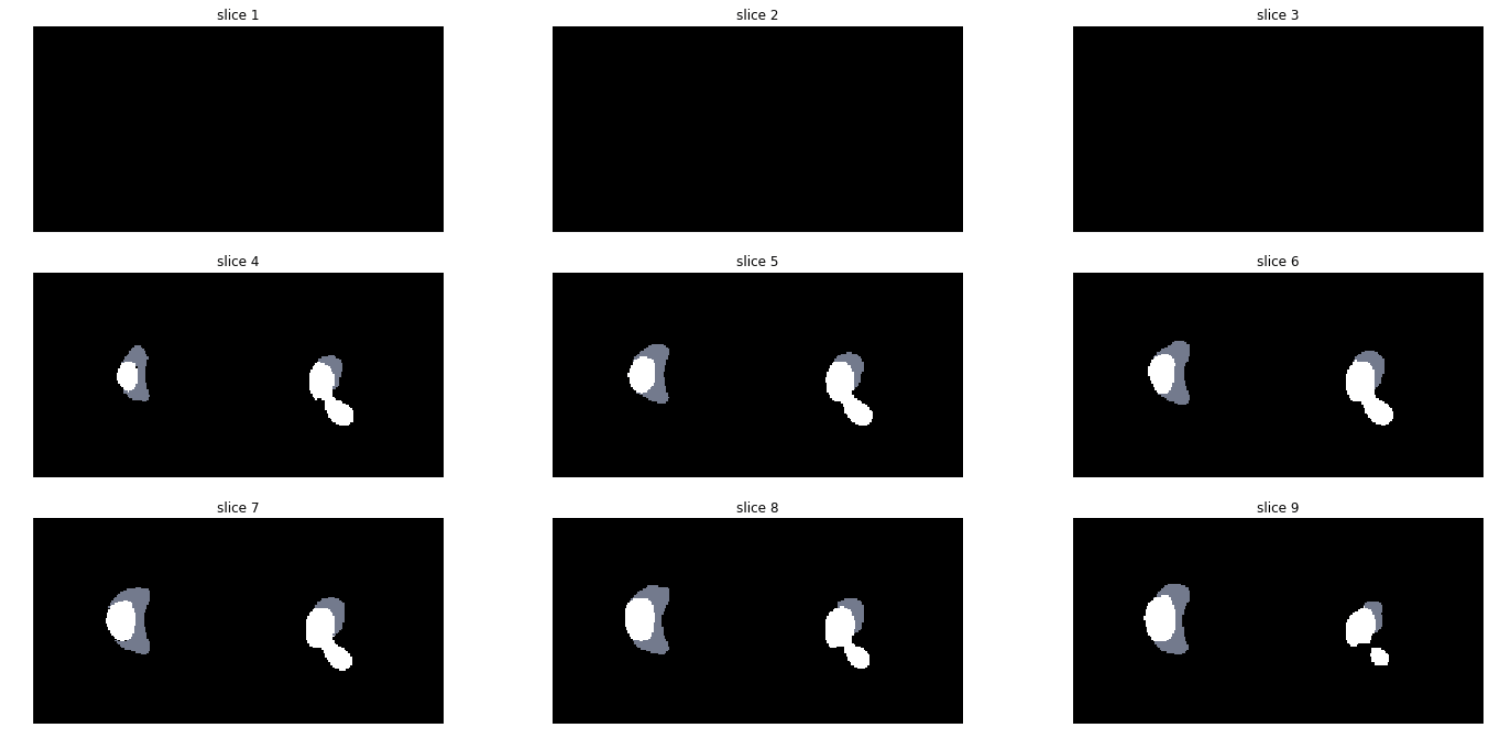
\includegraphics[width=\textwidth]{base_model2.png}
	\caption{Base model predictions. True segmentation is on the left, prediction on the right.}
	\label{fig:fig1}
\end{figure}

\begin{figure}[ht]
	\centering
	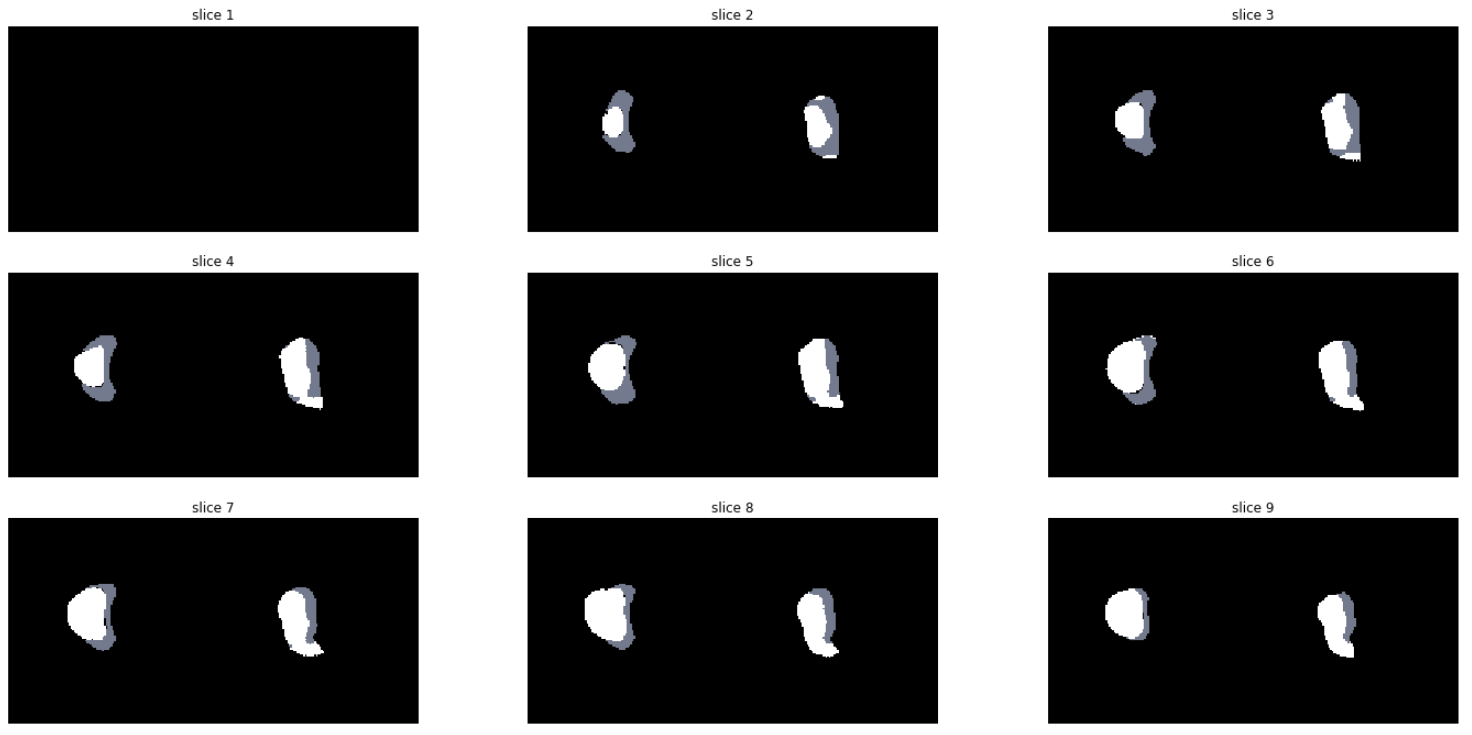
\includegraphics[width=\textwidth]{deeper_model2.png}
	\caption{Deeper model predictions. True segmentation is on the left, prediction on the right.}
	\label{fig:fig2}
\end{figure}

\section{Future work}

Besides the obvious polishing touches (writing unit-tests, building Sphinx docs) I would focus on training these models further and invest time in implementing the authors' data augmentation pipeline. Furthermore, adding residual layers (see \href{https://github.com/zhengyang-wang/3D-Unet--Tensorflow}{here} for example) to this architecture seems like a good idea that could further boost its utility and performance. Finally, I would love to \href{https://github.com/tensorflow/tensorboard/issues/227}{track the confusion matrix} using \texttt{tensorboard} in real-time while training.



\printbibliography

\end{document}
